% !TeX spellcheck = ru_RU
% !TEX root=../main.tex

\begin{lecture}[Буферные системы]
	\begin{lecSection}[Буферная емкость]
			\begin{definition}
			Водородный показатель: $pH = -\mathrm{lg}\left[\mathrm{H^+}\right]$.
		\end{definition}
	\begin{center}
	Рассмотрим буферную систему:
	\par $\mathrm{H_2CO_3 \rightleftharpoons H^+ + HCO_3^-}$
	\par $ \mathrm{OH^- + H_2CO_3 \rightarrow H_2CO_3^- + H_2O}$
	\par $ [HA]_0 = a $, $ [HOH]_0 = b $
	\par Из предыдущей лекции:
	\par $	K_A = \dfrac{[H^+] [A^-]}{[HA]}$
	\par $b = \dfrac{a K_A}{K_A + [H^+]} - [H^+] + \dfrac{ K_w }{ [H^+] }$
	\end{center}
	\begin{definition}
		Буферная емкость системы: $\beta = \dfrac{db}{d(pH)} = \dfrac{1}{d(pH)}{db}$.
	\end{definition}
	\begin{center}
	$[H^+] = x, \beta = \dfrac{db}{dpH} = \dfrac{db}{dx} \cdot \dfrac{dx}{dpH} = \dfrac{db}{dx} \cdot \dfrac{1}{\dfrac{dpH}{dx}}$
        \par $\dfrac{dpH}{dx} = - \dfrac{d}{dx}\left( \dfrac{1}{2,3}\mathrm{ln}x \right)  = - \dfrac{1}{2,3x}$
	\par $\beta = \dfrac{db}{dpH} = 2,3\dfrac{a K_A[H^+]}{(K_A + [H^+])^2} + [H^+] + \dfrac{ K_w }{ [H^+] }$
	\par $\beta = \dfrac{db}{dpH} \simeq 2,3 \dfrac{a K_A[H^+]}{(K_A + [H^+])^2}$
	\par Найдем максимум буферной ёмкости: $\dfrac{d\beta}{d[H^+]} = 0$
	\par $2,3aK_A\left(\dfrac{1}{(K_A+[H^+])^2}-\dfrac{2[H^+]}{(K_A + [H^+])^3}\right) = 0 \rightarrow 1-\dfrac{2[H^+]}{K_A + [H^+]} = 0$
	\par $\rightarrow K_A = [H^+] \rightarrow pH = pK_a$
	\par $\beta_{max} = \dfrac{2,3}{4}a \simeq \dfrac{a}{2}$, $K_A = [\mathrm{H^+}]$
	\par Реально в системе $(pK_a - 1) \leq pH \leq (pK_a + 1)$, например $pH = 3 \rightarrow 2 \leq pK_a \leq 4$.
	\end{center}
	\begin{figure}[H]
	\begin{minipage}[h]{0.26\linewidth}
		\centering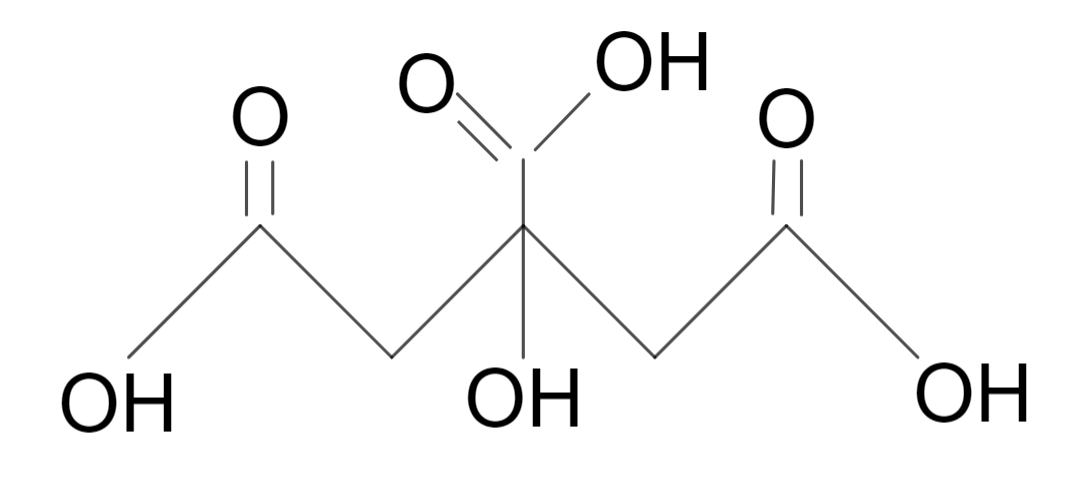
\includegraphics[width=\linewidth]{lecture_05/pic1}
			\caption{$pK_A = 3,13$}
	\end{minipage}
	\hfill
	\begin{minipage}[h]{0.30\linewidth}
		\centering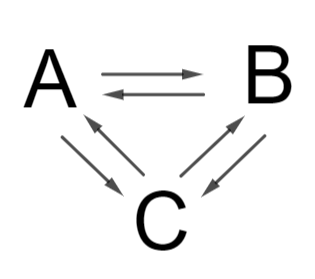
\includegraphics[width=\linewidth]{lecture_05/pic2}
			\caption{Схема Ларса Анзагера установления равновесия}
	\end{minipage}
	\hfill
	\begin{minipage}[h]{0.28\linewidth}
		\centering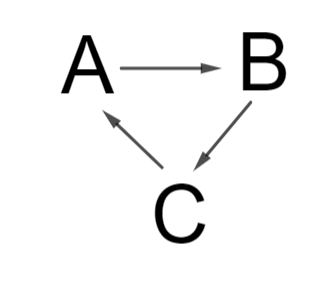
\includegraphics[width=\linewidth]{lecture_05/pic3}
		\caption{В равновесии так не бывает}
	\end{minipage}

	\end{figure}
	$\Delta G_s = \Delta G_d + \Delta G_{vw} + \Delta G_{cav}$, $\Delta G_{vw} + \Delta G_{cav} \simeq 10 \dfrac{\text{кДж}}{\text{моль}}$.
	\end{lecSection}
	
\end{lecture}